\chapter{Motivation} \label{cha:motivation}
Communicating intent and knowledge through visual means is maybe one of the most distinct features that separates humans from other animals.  Our ability to intuitively understand abstract representations created by other humans from distant places or times has shaped the world's history in unimaginable ways.  The fundamental goal of these representations~--~converying information~--~has not changed in the time between the earliest cave paintings 40000 years ago (Figure~\ref{fig:motivation:vis:cave}) and modern visualizations (Figure~\ref{fig:motivation:vis:modern}).  Humanity's focus on visual representations come from the fact that we are exceptionally good at intepreting visual language by dedicating a large portion of our brain to this task.  While other channels might be more effective at accessing emotional information, the visual cortex is the most effective way to ingest information.  This is part of the reason why our cultures have spent so much effort and time on perfecting visual languages and metaphors.  However, an image can never contain the full information and, as such, a good visualization is like a story; the author provides all the necessary components, but the final assembly occurs in the beholder and is thus subjective.

Good visualizations make subconcious use of one of the remarkable aspects of human perception.  We are capable of analyzing scenes both preattentively as well as attentively.  Preattentive perception happens when features of an image \emph{pop out}, or are obvious to the beholder without conscious effort.  This characterization is performed preattentively and largely independent of the number of objects that are involved.  Figure~\ref{fig:motivation:gestalt} shows an example of this effect using the Gestalt theory~\cite{wertheimer1922untersuchungen}.  In his work, Wertheimer found that attributes like closure, similarity, or continuation enable an observer to perceive a collection of objects as a continuous form (or \emph{Gestalt}).  He also investivated what objects can be added to these groupings before the continuous form is destroyed. 

\begin{figure}
  \centering
  \begin{subfigure}{0.4\textwidth}
    \fbox{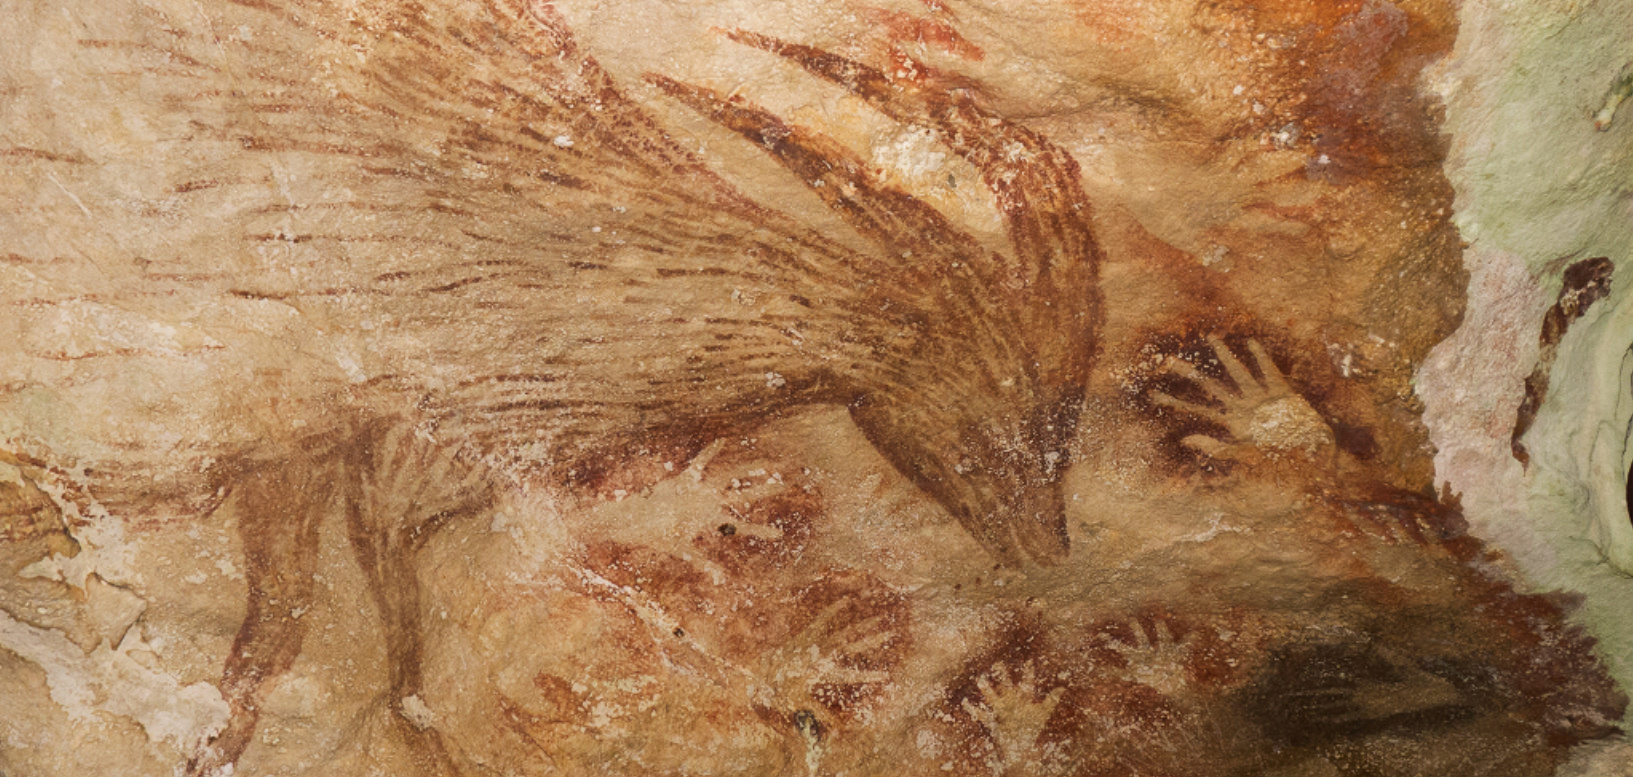
\includegraphics[width=\textwidth]{figures/motivation/cave.jpg}}
    \caption{The earliest known human cave painting from around 38000 BCE. Image copyright by Maxime Aubert. Re-printed with permission.}
    \label{fig:motivation:vis:cave}
  \end{subfigure}
  ~
  \begin{subfigure}{0.4\textwidth}
    \fbox{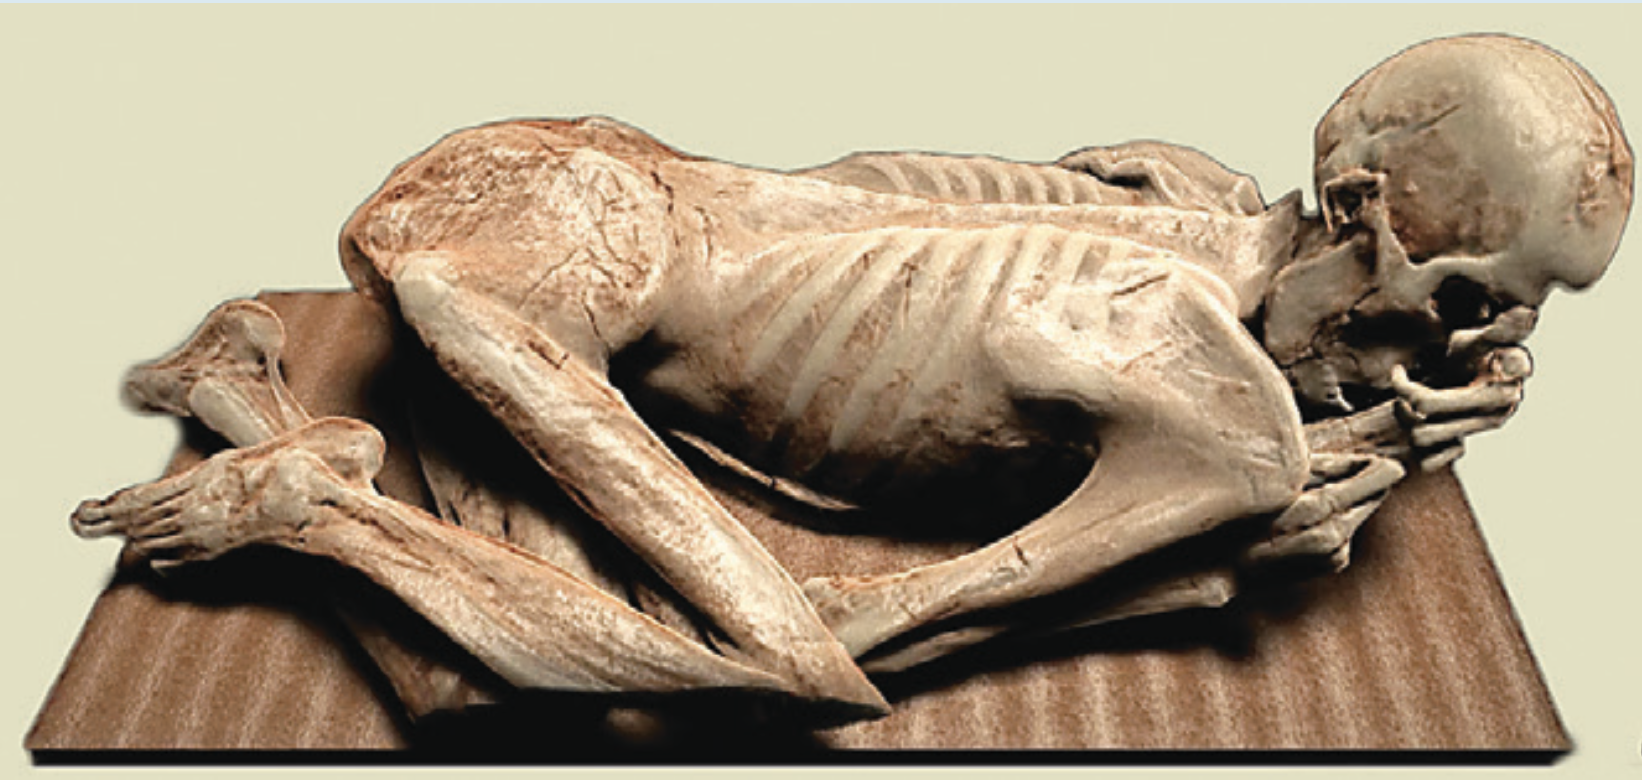
\includegraphics[width=\textwidth]{figures/motivation/gebelein.png}}
    \caption{A visualization using modern techniques of a pre-dynastic Egyptian mummy. Image copyright by Daniel J\"onsson. Re-printed with permission.}
    \label{fig:motivation:vis:modern}
  \end{subfigure}
  \caption{Two examples of human visualizations that are 40000 years apart. While the technologies changed drastically, the purpose of conveying information remains the same.}
  \label{fig:motivation:vis}
\end{figure}

\begin{figure}
  \centering
  \begin{subfigure}{0.4\textwidth}
    \fbox{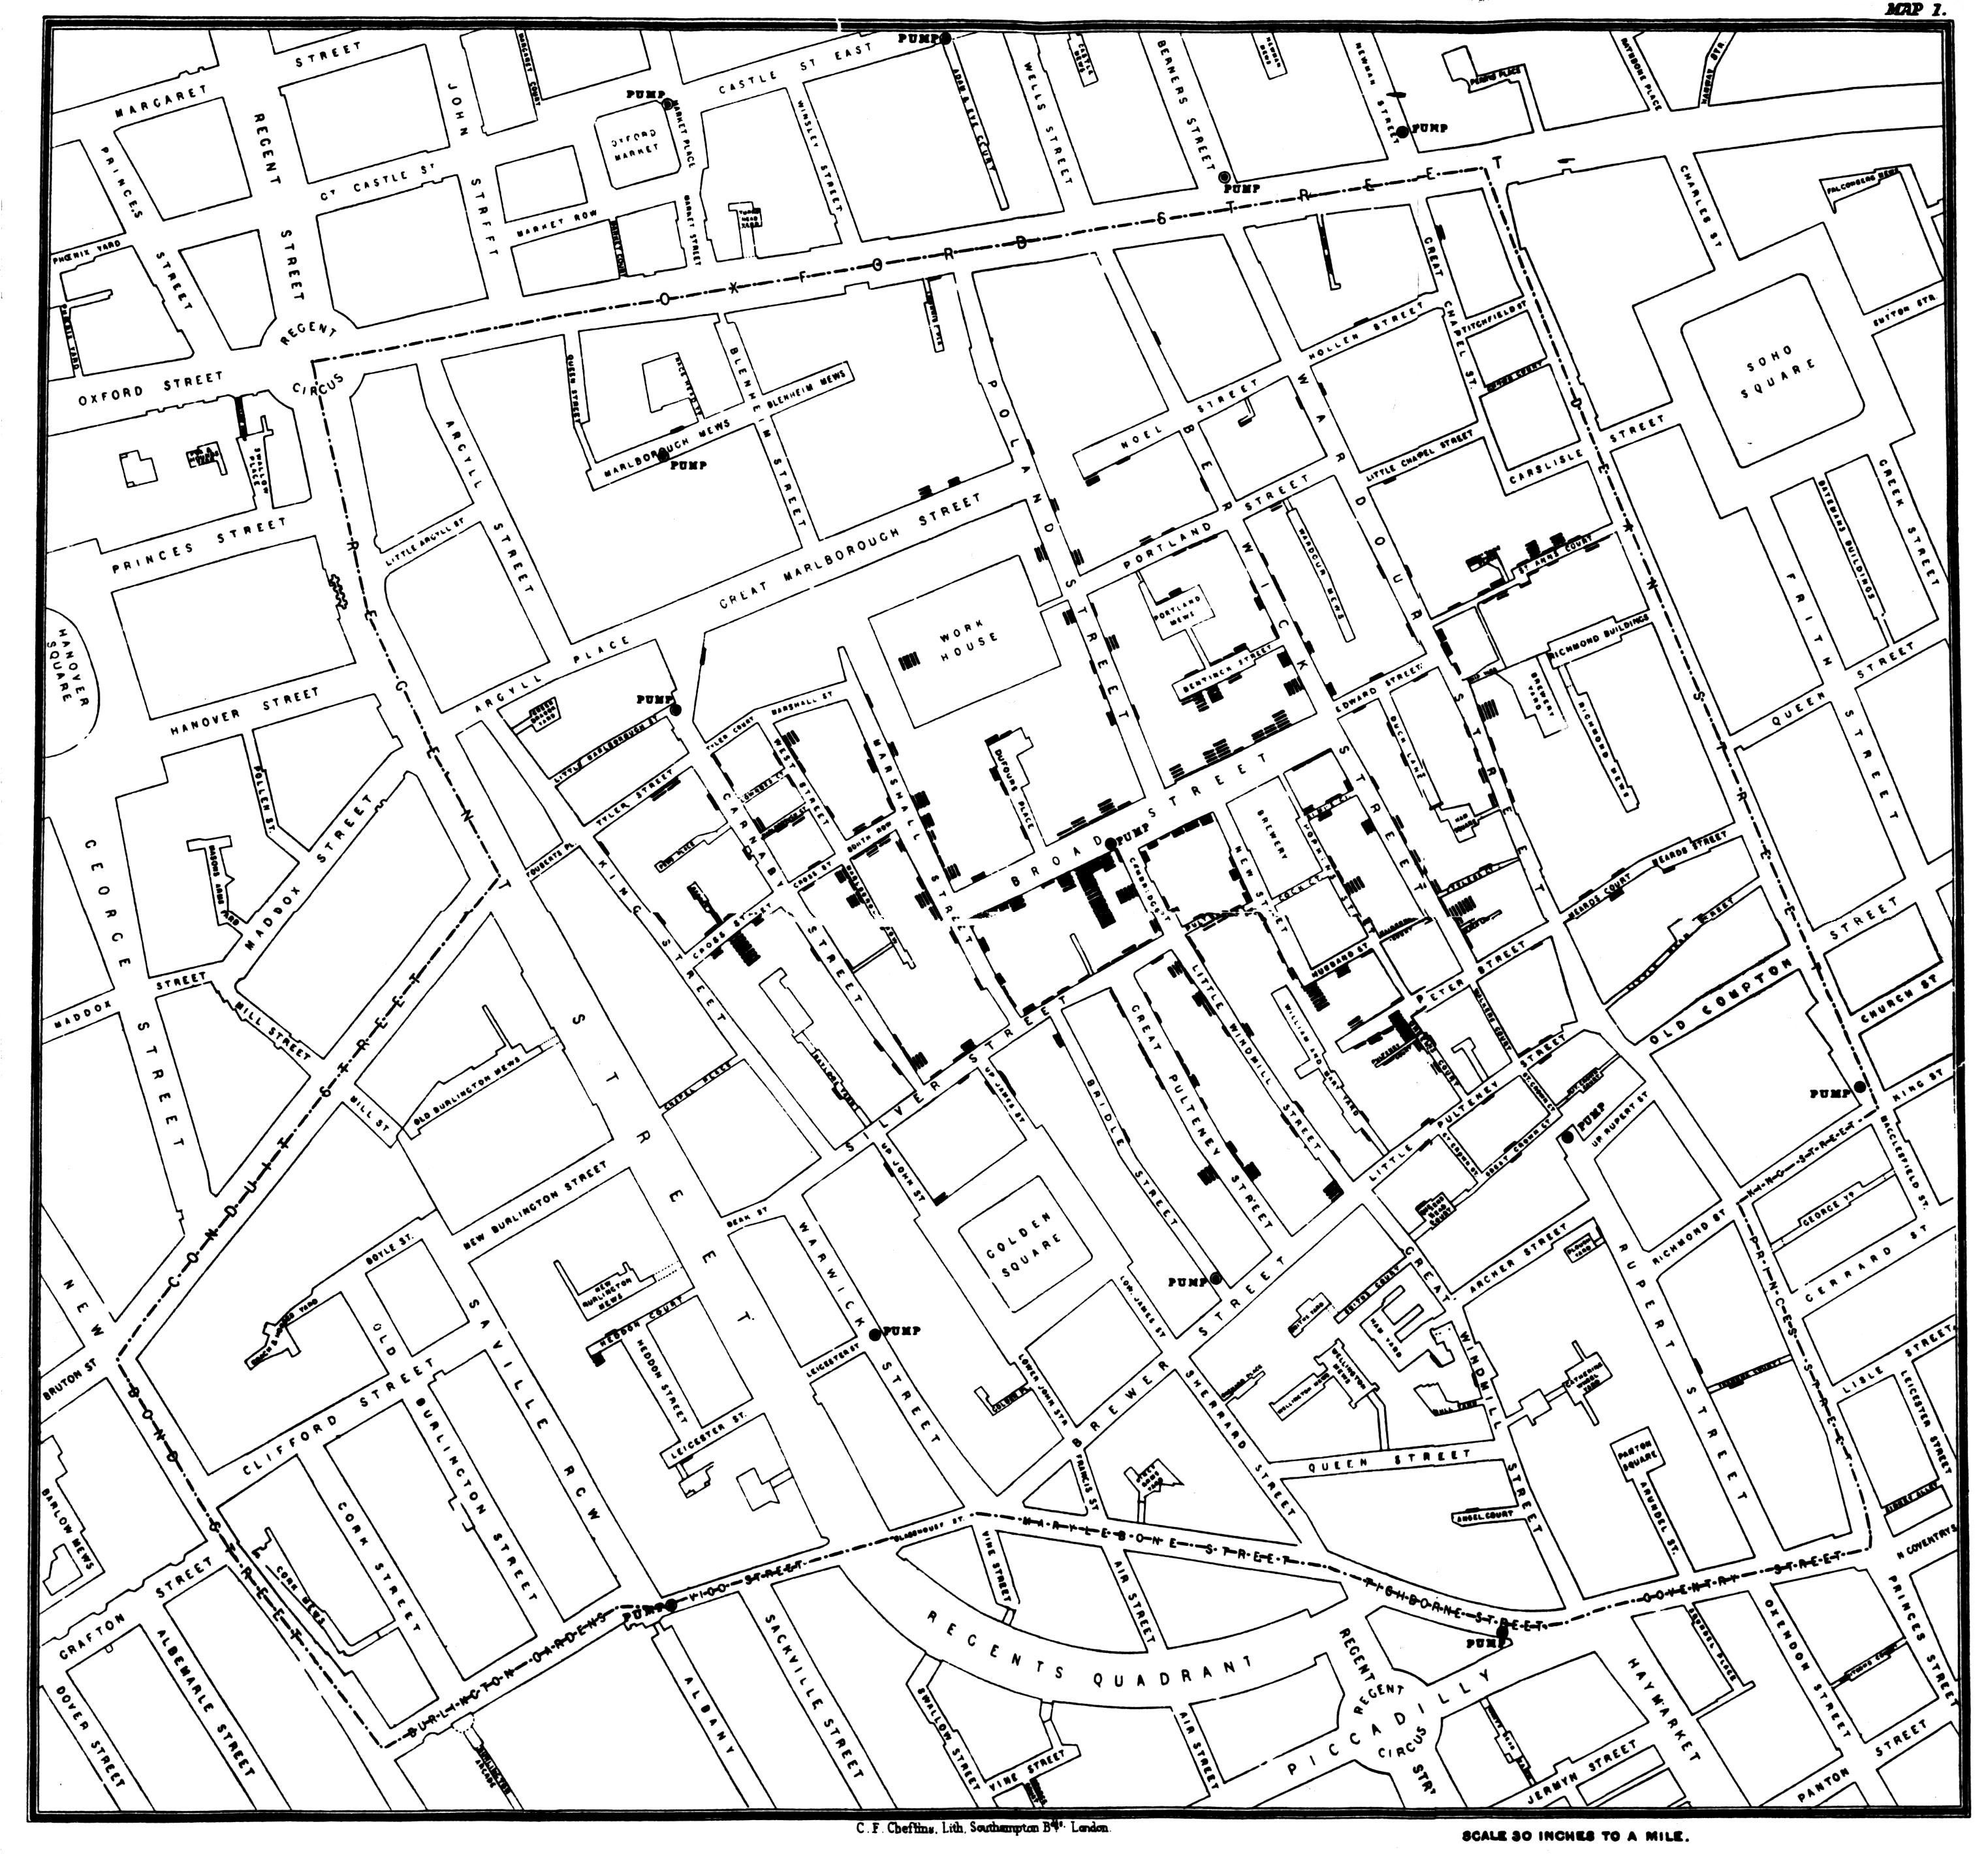
\includegraphics[width=\textwidth]{figures/motivation/cholera.jpg}}
    \caption{A spatial visualization of cholera outbreaks aruond Broad Street in London in 1854.}
    \label{fig:motivation:example:cholera}
  \end{subfigure}
  ~
  \begin{subfigure}{0.4\textwidth}
    \fbox{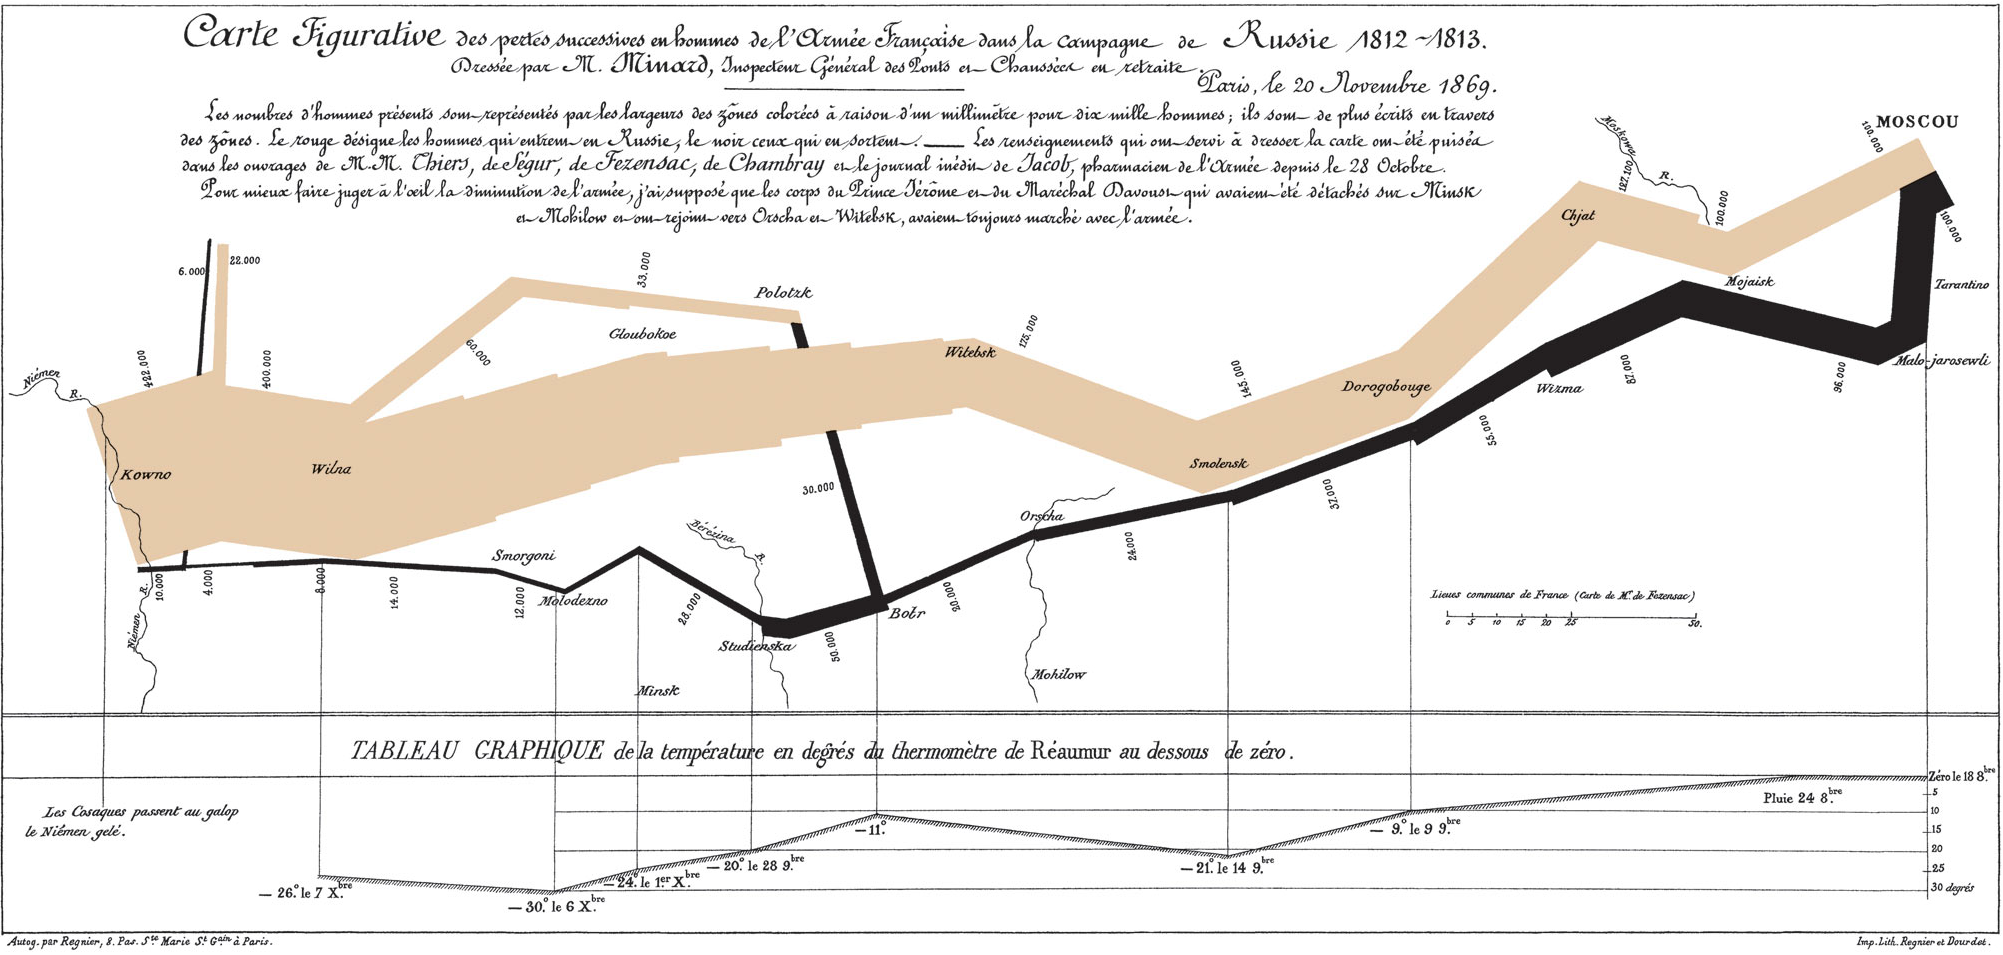
\includegraphics[width=\textwidth]{figures/motivation/napoleon.png}}
    \caption{A multivariate visualization of Napoleon's reteat from Moscow in 1812-1813.}
    \label{fig:motivation:example:napoleon}
  \end{subfigure}
  \caption{Two well-known examples of visualization used to produce scientific insight (Figure~\ref{fig:motivation:example:cholera}) and inform the general public about complicated data (Figure~\ref{fig:motivation:example:napoleon})}
  \label{fig:motivation:example}
\end{figure}

A good early example of the successful use of visualization is a spatial map of the cholera outbreaks around Broad street in London in 1854 (Figure~\ref{fig:motivation:example:cholera}).  The prevelant theory at the time for transmission of diseases was miasmatic and not caused by germs.  John Snow marked all cholera cases on a map and used this visualization to pinpoint the origin of the outbreak --- an infected pump~\cite{snow1855mode}.  While this visualization seems simple by today's standards, it was an additional important step towards establishing the germ theory of diseases.  Many decades before its official discovery, Snow already made use of the Gestalt theory to gain insights about the spatial distribution of cholera cases and relate them to the locations of the pumps in the area of London.  This is a clear example of a knowledge-driven approach, where a visualization is used to test a hypothesis and make sense of the available data.  Another example was created by Charles Joseph Minard in 1861 to visualize Napoleon's retreat from Moscow in 1812 (Figure~\ref{fig:motivation:example:napoleon}).  The map shows six different variables: geography, time, temperature, the Napoleon’s movement, and the remaining number of troops.  The layout and design and its ability to show Napoleon's terrible fate in Russia has caused this graphic to be called ``the best statistical graphic ever drawn''~\cite{tufte1983visual}.  As this data was produced from previously published work and mainly aimed at the general public, it serves as an example as to how visualization can be used to explain highly complex data to a public that possibly only has cursory knowledge about the topic.  Besides these two examples, Tufte, in his books, provides many more good examples of visualization mixing design and information reprensentation~\cite{tufte1991envisioning}.  All of these examples show an important difference in purpose between visualization and computer graphics, which is also exemplified in Ben Shneiderman's quote that ``the purpose of visualization is insight, not pictures''.  Instead of generating images devoid of information, the purpose of visualization is to create images that enable a person to derive insight.

\begin{figure}
  \centering
  \fbox{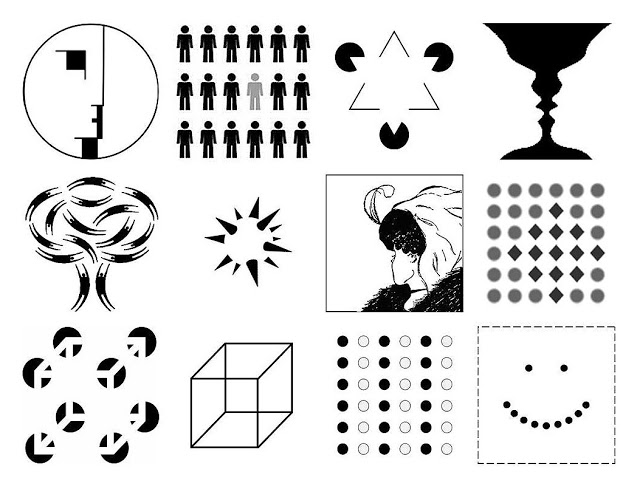
\includegraphics[width=\textwidth]{figures/motivation/gestalt.jpg}}
  \caption{Examples of Gestalt theory $\cdots$ Change image}
  \label{fig:motivation:gestalt}
\end{figure}

\section{Applications}
As alluded to in the two examples provided above, visualization cannot occur realistically when a specific \emph{target domain} or \emph{problem domain} is considered.  Except basic research, all visualization research has to take the domain into account and is meaningless on its own.  Even for basic research, its effectiveness is important and has to be proven.  The different domains are frequently tackled with visualization applications that are tailored to a \emph{domain expert}, who is interested in understanding a specific aspect of their data.  The design of a visualization application requires knowledge from many different fields, such as computer science, perception, cognition, interaction design, or art, and is thus in itself multidisplinary~\cite{mccormick1987visualization}.  The design process furthermore requires in-depth knowledge about the domain and therefore demands interdisciplinary collaborations with experts from other fields~\cite{kirby2013visualization}.

Over the past years, the field of visualization has matured to the degree that basic research on novel visualizatoin techniques is being replaced with application-driven research that applies the generic toolset the community has acquired.  Even though most problems require a custom solution to some extent, it is still possible for the visualization community as a whole to benefit from the reasearch on individual applications as they feed back into the general knowledge base.  This feedback loop, combined with the insight that custom solutions are required for the majority of non-trivial tasks, excluded the use of ready-made programs as well.


%\todo{Anders: You can not express your views and opinions} Almost every applied scientific field has a founding principle without which the field as a whole loses its meaning. In Physics, every discovery must, at least in principle, be experimentally verifiable. Mathematical proofs have to be logically consistent. The same holds true to the field of Visualization, which could not exist without the collaboration between domain experts and visualization researchers. Unlike other scientific fields where interdisciplinary is a beneficial aspect of research, it is an essential component that every visualization research directly or indirectly can be traced to a knowledge consumer that is aided by said research. If this does not hold true for a piece of research, the boundary between Visualization research and Computer Graphics research is blurred.

%Throughout the work that has led to this thesis, I have collaborated with domain experts from many different fields, producing tailored visualization applications that both supported their discoveries as well as providing contributions to the field of visualization. The topic of this thesis is to provide an overview of the lessons learned when designing scientific visualization applications in close collaboration with domain experts from widely varying fields, exemplified in some of my collaborations over the past 6 years.

%In my experience, the interactions between visualization expert and domain expert usually progress along different phases and are typically cyclic in nature; each iteration building on the previous ones to work towards a final application. Most collaborative projects follow a similar structure and can be broadly grouped into two categories:

%1. Type I: Expert-initiated. In this case, a domain expert usually has a series of datasets and hypotheses, but they are lacking the knowledge or tools to gain insight from the data. They then contact a visualization researcher with a more-or-less concrete list of questions that they would like to answer or have answered.
%2. Type II: Visualization-initiated. In this case, a visualization expert is introduced to a domain scientist's data and discovers the possibility of applying visualization techniques without the domain expert having a specific a priori question. This usually occurs with data that is unique and interesting in some sense and, if successful, usually generated questions that the domain experts did not even think of asking before. However, this type of collaboration sometimes suffer from the "finding a problem" dilemma in which interesting data is present, but there is not much visualization research to be gained from dealing with the data

%The usual workflow of both types of collaborations is the following:
%1. Initial contact: Depending on the category of collaboration this is initiated by either the domain expert or the visualization researcher and consists of a cursory introduction into each others fields. The domain scientist provides a limited introduction into the they research topic and the visualization expert brainstorms various techniques that might prove beneficial.
%2. Data retrieval: The first step to every collaboration is the development of interfacing techniques. Usually, visualization researchers have access to a growing toolkit of visualization techniques int which the domain experts data has to be imported. In some cases, this might be trivial (for example, loading RAW data), whereas other cases might prove more difficult (for example, converting between grids)
%3. Feasibility study: Usually at this step, the visualization researcher has to assess whether there is any potential research in the collaboration. This step is probably one of the most challenging ones as the goals of the different parties might diverge. A novel visualization technique that might be beneficial to the visualization researcher might not be accepted by the domain scientist, complicating the collaboration. This step is furthermore complicated by the fact that some projects do not have an initial payoff in novel visualization techniques, but have the promise of future benefits once an initial collaboration is established. 
%4. Application design: In this step, the visualization researcher and the domain expert collaborate in varying degrees on designing the application. On the visualization side, this consists of attaining a cursory knowledge of the subject matter as well as developing the application itself. On the domain expert side it consists of providing knowledge about his field, experimenting with the software, and providing feedback.
%5. Publish results: The results of the collaboration are published in both the visualization field as well as the scientific domain of the expert.

%For a single project, phase 4 is usually repeated a number of times with constant feedback between the visualization expert and the domain scientist. These iterative refinement steps are useful as in most cases, the expectations of the application can be very different between the two parties and can be bridged by these feedback sessions.

%This 5 phase model naturally is only a broad description of a complicated social process, but can serve as the basis for the following discussions. Multiple questions arise in this context that have to be addressed:
% 1. Does the project provide any foundation for good scientific visualization research?
% 2. How to structure the interaction between researcher and domain expert? How much interaction is too much? How little is too little?
% 3. When to break the cycle of iterative improvements? How to detect when a "good enough" result has been achieved in \#4?
% 4. What are the benefits and drawbacks of including a sixth phase for "going the extra mile" when it comes to improving an application beyond the point of paper-usability? Should this be considered part of the Visualization research and should researchers get credited for it?


% - Usefulness of convincing a domain expert of the usefulness of a visualization technique.
% - Obviously, there are visualization techniques that are not intuitively understandable, but useful nontheless
% - For example: Parallel coordinates plot [USAR evaluation]

%- What is visualization
% - Sitting between computer graphics and the application domains
% - "Computer Graphics with a purpose"
% - Lots of cross-talk between computer graphics papers and visualization papers [A-Buffer paper]

%- Seeing visualization as a service rather than a stand-alone science
% - Problems between delivering an application vs developing a fully fledged product
% - Getting recognition when papers are published in domain fields
% - Engineering efforts to make it more usable
% - Visualization researchers cannot be the code monkeys of other fields

%- Ability to get recognition for public outreach
% - "Publish and perish": Case that even though papers are published, having a public outreach might reach many more people
% - [New Horizons]

%- User studies
% - Domain expert needs to be involved in finding the peope that want to participate in a study
% - How do you deal with the requirement of a user study in very limited field? [Space Weather]

%- Visualization as a teaching tool
% - Targeting not domain scientists, but the public audience at large
% - [3D Interaction gestures]

%- Design circles
%- Finding visualization challenges in seemingly trivial fields

%- Different types of applications
%  - Initial information gathering
%  - Applying the same techniques to more datasets

%- The purpose of visualization is insight, not pictures” (McCormick et al. 1987)
%- Explaning multiviews, brushing, linking, etc (Tory 2003)
%- Volume rendering integral  (Max 1995)

%- Cultural component in understanding visualizations